% document formatting
\documentclass[10pt]{article}
\usepackage[utf8]{inputenc}
\usepackage[left=1in,right=1in,top=1in,bottom=1in]{geometry}
\usepackage[T1]{fontenc}
\usepackage{xcolor}

% math symbols, etc.
\usepackage{amsmath, amsfonts, amssymb, amsthm}
\usepackage{mathtools}

% lists
\usepackage{enumerate}

% images
\usepackage{graphicx} % for images
\usepackage{multirow}

% code blocks
\usepackage{minted, listings} 

% verbatim greek
\usepackage{alphabeta}

\graphicspath{{./assets/images}}

\newcommand{\solution}{\textbf{Solution:}} 
\newcommand{\example}{\textbf{Example: }}
\newcommand{\sinc}{\text{sinc}}
\newcommand{\rect}{\text{rect}}
\newcommand{\llra}{\Longleftrightarrow}
\newcommand{\fourier}{\mathcal{F}}
\newcommand{\absint}{\int_{-\infty}^\infty}
\newcommand{\dd}{\text{d}}

\title{EC ENGR 102 Week 7}

\author{Aidan Jan}
\date{\today}

\begin{document}
\maketitle

\section*{Fourier Transform Pairs}
\begin{align*}
    \rect(t/T) &\llra T \sinc(\omega T/2\pi)\\
    e^{at}u(t) &\llra \frac{1}{a + j\omega}\\
    \fourier\left[e^{a\lceil t \rceil}\right] &= \frac{2a}{a^2 + \omega^2}\\
    \sinc(t/2\pi) &\llra 2\pi \rect(\omega)\\
    \triangle(t) &\llra \sinc^2(\omega/2\pi)\\
    \fourier[\sinc^2(t)] &= \triangle(\omega / 2\pi)\\
    \Aboxed{\delta(t) &\llra 1}\\
    \Aboxed{\delta(t - \tau) &\llra e^{-j\omega \tau}}\\
    \Aboxed{1 &\llra 2\pi \delta(\omega)}\\
    \Aboxed{u(t) &\llra \pi \delta(\omega) + \frac{1}{j\omega}}\\
    \Aboxed{e^{j\omega_0 t} &\llra 2\pi \delta(\omega - \omega_0)}\\
    \Aboxed{\cos(\omega_0 t) &\llra \pi(\delta(\omega - \omega_0) + \delta(\omega + \omega_0))}\\
    \Aboxed{\sin(\omega_0 t) &\llra j\pi(\delta(\omega + \omega_0) - \delta(\omega - \omega_0))}
\end{align*}

\subsection*{Fourier Transform of a constant}
What, intuitively, should the Fourier transform of $f(t) = 1$ be?\\\\
Lets try to evaluate it using the definition of the Fourier transform.

\begin{align*}
    \fourier[1] &= \absint e^{-j\omega t} \dd\\
    &= \left.\frac{e^{-j\omega t}}{-j\omega}\right|^{\infty}_{-\infty}
\end{align*}
We run into a problem here: we cannot evaluate this integral.  Instead, we use duality.  We know that $\delta(t) \llra 1$, and therefore by duality, we have that
\[\boxed{1\llra 2\pi \delta(\omega)}\]
This confirms our intuition: 1 is a constant, and therefore, its spectrum should only have a DC component (i.e., at $\omega = 0$).

\subsection*{Fourier transform of a modulated signal}
A major component of communications has to do with \textit{modulation}.  For example, AM and FM radio are amplitude modulation and frequency modulation respectively.  AM radio involves multiplying $f(t)$, the signal you wish to transmit, with a complex exponential at a carrier frequency, $\omega_0$.  This frequency, $\omega_0$, is the frequency you dial in your car to get AM radio.\\\\
Here are three ways to modulate a signal: If $\fourier[f(t)] = F(j\omega)$, then
\begin{align*}
    \fourier[f(t) e^{j\omega_0 t}] &= F(j(\omega - \omega_0))\\
    \fourier[f(t) \cos(\omega_0 t)] &= \frac{1}{2}(F(j(\omega - \omega_0)) + F(j(\omega + \omega_0)))\\
    \fourier[f(t) \sin(\omega_0 t)] &= \frac{1}{2j} (F(j(\omega - \omega_0)) - F(j(\omega + \omega_0)))
\end{align*}
Typically, modulation is done through multiplication by $\cos(\omega_0 t)$.  Modulation is dual to the time shift Fourier transform.\\\\
What modulation intuitively does is take $F(j\omega)$ and create replicas at $\pm \omega_0$.

\subsection*{Fourier Transform of a Complex Exponential}
If the $\delta$ function is shifted in frequency,
\begin{align*}
    \fourier^{-1}[\delta(\omega - \omega_0)] &= \frac{1}{2\pi} \absint \delta(\omega - \omega_0) e^{j\omega t} \dd \omega\\
    &= \frac{1}{2\pi} e^{j\omega_0 t}
\end{align*}
so,
\[\boxed{e^{j\omega_0 t} \llra 2\pi \delta(\omega - \omega_0)}\]

\subsection*{Fourier Transform of Cosine}
Now that we know the Fourier transform of the complex exponential, we can derive the Fourier transform of cosine and sine.  Recall that
\[\cos(\omega_0 t) = \frac{1}{2} \left(e^{j\omega_0 t} + e^{-j\omega_0 t}\right)\]
and therefore,
\begin{align*}
    \fourier[\cos(\omega_0 t)] &= \fourier\left[\frac{1}{2} \left(e^{-j\omega_0 t} + e^{j\omega_0 t}\right)\right]\\
    &= \frac{1}{2} \left(\fourier\left[e^{j\omega_0 t}\right] + \fourier\left[e^{-j\omega_0 t}\right]\right)\\
    &= \frac{1}{2} (2\pi \delta(\omega - \omega_0) + 2\pi \delta(\omega + \omega_0))\\
    &= \pi(\delta(\omega - \omega_0) + \delta(\omega + \omega_0))
\end{align*}
The same can be done for sine.

\subsection*{Fourier transform of a step function}
\begin{align*}
    \fourier[u(t)] &= \absint u(t) e^{-j\omega t} \dd t\\
    &= \int_0^\infty e^{-j\omega t} \dd t\\
    &= \left.\frac{e^{-j\omega t}}{-j\omega}\right|_0^\infty
\end{align*}
and thus the integral doesn't converge.  Instead, we'll use an idea called limiting Fourier transforms.

\subsubsection*{Limiting Fourier Transforms}
When the Fourier transform integral doesn't converge, and there's not a "trick" we can use, an alternative approach is to use limiting Fourier transforms.  In this appraoch, we represent the signal as a limit of a sequence of signals for which the Fourier transforms do exist.  i.e., consider $f_n(t)$ which does have a Fourier transform.  If
\[f(t) = \lim_{n\rightarrow \infty}f_n(t)\]
then we also have that 
\[F(j\omega) = \lim_{n \rightarrow \infty}F_n(j\omega)\]
if the limit makes sense.

\subsubsection*{Limiting Fourier Transform Example}
Consider the Fourier transform of $f(t) = \text{sign}(t)$.  This signal is defined as:
\[f(t) = \begin{cases} 1 & t > 0 \\ 0 & t = 0 \\ -1 & t < 0\end{cases}\]
We previously derived the Fourier transform for $e^{-at} u(t)$.  We can use this signal to make a limiting approximation to $\text{sign}(t)$ by setting
\[f_a(t) = e^{-at} u(t) - e^{at}u(-t)\]
This is shown below:
\begin{center}
    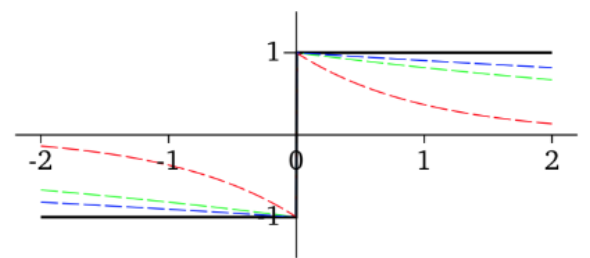
\includegraphics[scale=1]{W7_1.png}
\end{center}
We show $f_a(t)$ for $a = 1$ (red), $a = 1/5$ (green), and $a = 1/10$ (blue).\\
As $a\rightarrow 0$, then, $f_a(t) \rightarrow \text{sign}(t)$.\\\\
Hence, we can compute the Fourier transform, $F_a(j\omega) = \fourier[f_a(t)]$, and then compute the Fourier transform of $\text{sign}(t)$ as the limit of $F_a(j\omega)$ as $a \rightarrow 0$.
\begin{align*}
    F_a(j\omega) &= \fourier[f_a(t)]\\
    &= \fourier[e^{-at} u(t) - e^{at} u(-t)]\\
    &= \fourier[e^{-at} u(t)] - \fourier[e^{at} u(-t)]\\
    &= \frac{1}{a + j\omega} - \frac{1}{a - j\omega}\\
    &= \frac{-2j\omega}{a^2 + \omega^2}
\end{align*}
When $\omega = 0$, then $F_a(j\omega) = 0$ for any $a \neq 0$.  Otherwise, if $\omega \neq 0$, then
\begin{align*}
    \lim_{a \rightarrow 0} F_a(j\omega) &= \lim_{a \rightarrow 0} \frac{-2j\omega}{a^2 + \omega^2}\\
    &= \frac{-2j\omega}{\omega^2}\\
    &= \frac{2}{j\omega}
\end{align*}
With this, we can state that
\[\text{sign}(t) \llra \begin{cases} \frac{2}{j\omega} & \omega \neq 0 \\ 0 & \omega = 0\end{cases}\]
Now, the step function can be written in terms of the sign function, i.e.,
\[u(t) = \frac{1}{2} + \frac{1}{2} \text{sign}(t)\]
Therefore,
\begin{align*}
    \fourier[u(t)] &= \fourier\left[\frac{1}{2} + \frac{1}{2} \text{sign}(t)\right]\\
    &= \frac{1}{2}2\pi \delta(\omega) + \frac{1}{2} \left(\frac{2}{j\omega}\right)\\
    &= \pi \delta(\omega) + \frac{1}{j\omega}
\end{align*}
Note that the second term is zero at $\omega = 0$, and so the specturm of $u(t)$ is $\pi\delta(\omega)$ at $\omega = 0$.  Thus,
\[u(t) \llra \pi \delta(\omega) + \frac{1}{j\omega}\]

\subsection*{Fourier Transform of an Integral}
[FILL]
Now, with the Fourier transform of the step function, it is possible to calculate the Fourier transform of an integral.  Recall that we can represent integration as the convolution with the step function, i.e.
\[\int_{-\infty}^t f(\tau) \dd \tau = (f * u)(t)\]
Therefore,
\begin{align*}
    \fourier\left[\int_{-\infty}^t f(\tau) \dd \tau\right] &= \fourier[f(t)] \fourier[u(t)]\\
    &= F(j\omega)\left(\pi \delta(\omega) + \frac{1}{j\omega}\right)\\
    &= \pi F(0) \delta(\omega) + \frac{F(j\omega)}{j\omega}
\end{align*}
Therefore,
\[\boxed{\int_{-\infty}^t f(\tau) \dd \tau \llra \pi F(0) \delta(\omega) + \frac{F(j\omega)}{j\omega}}\]

\section*{Frequency Response}
We previously discussed the impulse response, $h(t)$, which is the output of a system when the input is an impulse, $\delta(t)$.  We saw that $h(t)$ characterized any LTI system, as for any LTI system with input, $x(t)$, we could calculate the output as 
\begin{align*}
    y(t) &= (x * h)(t)\\
    &= \absint x(\tau) h(t - \tau) \dd \tau
\end{align*}
A complication we discussed is that computing the output this way requires evaluating a convolution integral, which can be difficult and time-consuming.\\\\
But now, equipped with the convolution theorem, why not just take the Fourier transform of both sides?  This turns the convolution into multiplcation.
\[Y(j\omega) = H(j\omega)X(j\omega)\]
where $X(j\omega)$ is the Fourier transform of the input, $Y(j\omega)$ is the Fourier transform of the output, and $H(j\omega)$ is the \textit{frequency response}, i.e., the Fourier transform of the impulse response.\\

[FILL SCREENSHOTS OF RC CIRCUIT DRAWINGS (LECTURE 13)]

[this stuff won't be tested]

\begin{itemize}
    \item In addition to \textit{frequency response}, $H(j\omega)$ is sometimes called the \textit{transfer function} of the system.
    \item The reason its called frequency response is that $H(j\omega)$ describes how the input is changed at every single frequency.
    \item In particular, the frequency response scales the amplitude response by $|H(j\omega)|$, i.e.,
    \[|Y(j\omega)| = |H(j\omega)||X(j\omega)|\]
    \item The frequency response shifts the phase response by $\angle H(j\omega)$, i.e.,
    \[\angle Y(j\omega) = \angle H(j\omega) + \angle X(j\omega)\]
\end{itemize}
To see this, note that if the input to a system is a complex exponential, $e^{j\omega_0}t$ (recall, these are the eigenfunctions of an LTI system), then
\begin{align*}
    X(j\omega) &= \fourier\left[e^{j\omega_0 t}\right]\\
    &= 2\pi \delta(\omega - \omega_0)
\end{align*}
Therefore, the output is
\begin{align*}
    Y(j\omega) &= H(j\omega)(2\pi \delta(\omega - \omega_0))\\
    &= H(j\omega_0)(2\pi \delta(\omega - \omega_0))
\end{align*}
This means that
\begin{align*}
    y(t) &= \fourier^{-1}[Y(j\omega)]\\
    &= \fourier^{-1}[H(j\omega_0)(2\pi \delta(\omega - \omega_0))]\\
    &= H(j\omega_0) e^{j\omega_0 t}\\
    &= |H(j\omega_0)| e^{j(\omega_0 t + \angle H(j\omega_0))}
\end{align*}
\begin{itemize}
    \item In the last step, we break $H(j\omega_0)$ into its magnitude and angle components.  The magnitude is the coefficient, the angle (in exponential form), when multiplied with the exponential gets added into the exponent.
\end{itemize}
To summarize here, we input a sinusoidal input, $x(t) = e^{j\omega_0 t}$ to a LTI system and saw that the output was
\[y(t) = |H(j\omega_0)| e^{j(\omega t + \angle H(j\omega_0))}\]

i.e., inputting a complex sinusoid to an LTI system produces an output that:
\begin{itemize}
    \item is at the same frequeny $\omega_0$
    \item is scaled in amplitude by $|H(j\omega_0)|$
    \item is phase shifted by $\angle H(j\omega_0)$
\end{itemize}

\subsection*{Frequency Response Example}
Consider the input:
\[x(t) = 2\cos(t) + 3\cos(3t/2) + \cos(2t)\]
and the system with impulse response
\[h(t) = \frac{2}{\pi} \sinc^2(t/\pi)\]
Find $y(t) = (x * h)(t)$.\\\\
Remember that the convolution becomes multiplication if we do the Fourier transform on it.\\\\
Converting $x(t)$ gives six impulse functions, and converting $h(t)$ gives a triangle function.  (Refer to the Fourier pairs at the top!)\\\\
Now, we can multiply them:
\begin{center}
    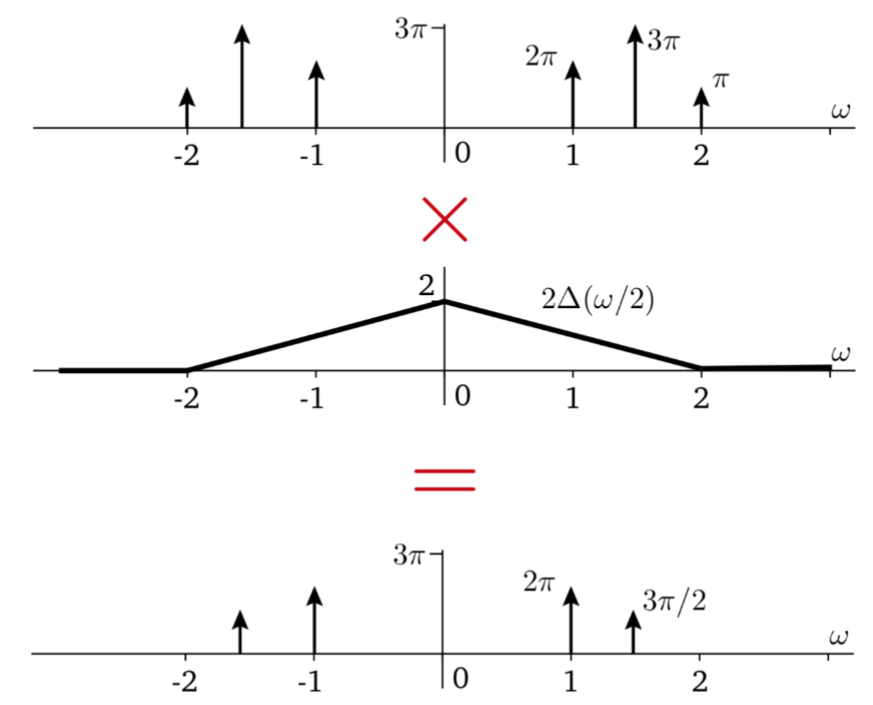
\includegraphics[scale=0.6]{W7_2.png}
\end{center}
The product (if you worked out the math) is 
\[Y(j\omega) = 2\pi[\delta(\omega - 1) + \delta(\omega + 1)] + \frac{3\pi}{2} [\delta(\omega - 3/2) + \delta(\omega + 3/2)]\]
Taking the inverse Fourier transform, we get that
\[y(t) = 2\cos(t) + \frac{3}{2} \cos(3t/2)\]

\subsection*{Frequency Response Example 2}
Let $x(t) = e^{-t} u(t)$.  We input this signal into a system with impulse response:
\[h(t) = 2e^{-2t} u(t)\]
What are $Y(j\omega)$ and $y(t)$?\\\\
\begin{align*}
    Y(j\omega) &= \frac{2}{(1 + j\omega)(2 + j\omega)}\\
    &= \left[\frac{A}{1 + j\omega} + \frac{B}{2 + j\omega}\right]
    \intertext{By partial fraction decomposition,}
    &= \frac{2}{1 + j\omega} - \frac{2}{2 + j\omega}
\end{align*}
Now, finish this problem by simply referring to the Fourier pairs.
\[y(t) = 2e^{-t} u(t) - 2e^{-2t}u(t)\]
Recall that when we multiply two complex numbers, their magnitudes multiply and their phases add.  This is shown below:
\begin{center}
    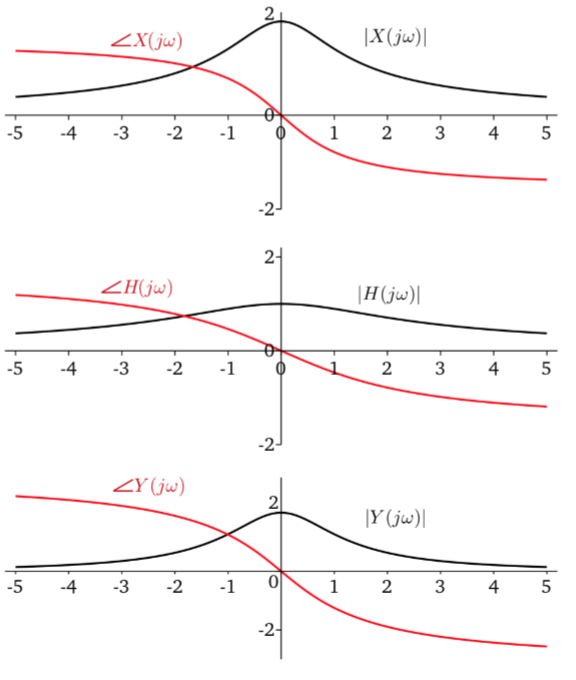
\includegraphics[scale=0.7]{W7_3.png}
\end{center}
To measure the frequency response of an LTI system, we can input complex exponentials different frequencies.
\begin{itemize}
    \item At the output we measure change in amplitude, giving $|H(j\omega)|$.
    \item We also measure the phase shift, giving the phase of $H(j\omega)$.
    \item This describes the entire LTI system!
\end{itemize}

\subsection*{Filters}
Filters are designed to extract or attenuate certain desired frequencies from a signal.  For example, consider a recording of music where the microphones accidentally recorded the sopranos too loudly. It would be possible to rebalance the audio by attenuating higher frequencies in the signal.\\\\
We'll first discuss ideal filters, which only pass through certain frequencies.  There are three main types of filters we'll discuss:
\begin{itemize}
    \item Low pass filter: suppresses all frequencies that are higher than a specified frequency, $\omega_c$.  Its name comes from the fact that it lets frequencies less than $\omega_c$ through.  (i.e., low frequencies)
    \item High pass filter: suppresses all frequencies that are lower than a specified frequency, $\omega_c$.
    \item Band pass filter: suppresses all frequencies outside of a range $\pm \omega_c$ around a chosen frequency $\omega_0$.
    \item These three filters are illustrated below.
\end{itemize}
\begin{center}
    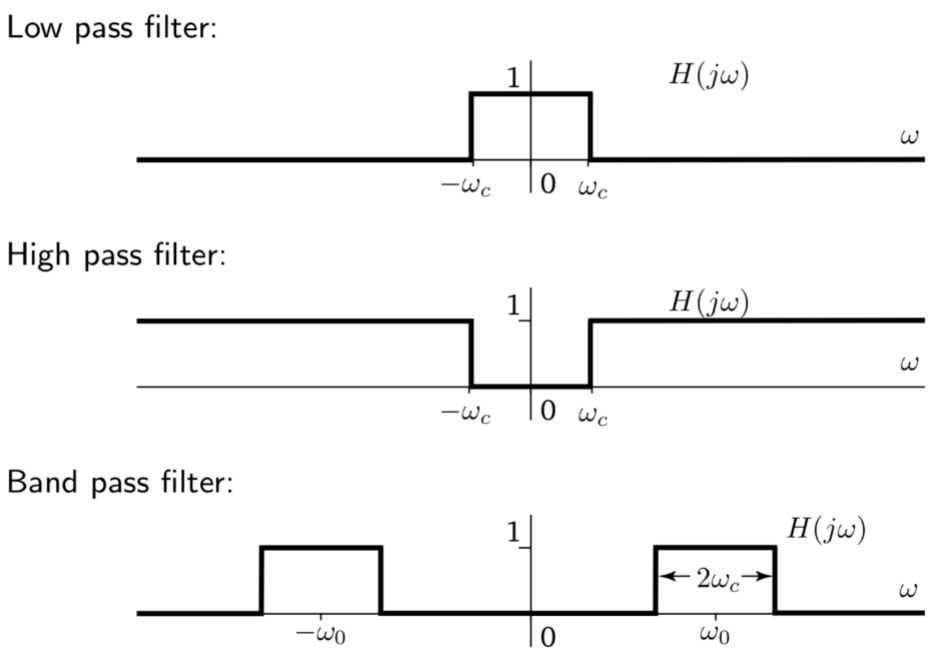
\includegraphics[scale=0.8]{W7_4.png}
\end{center}

\subsubsection*{Ideal Low Pass Filter}
The ideal low pass filter is
\begin{center}
    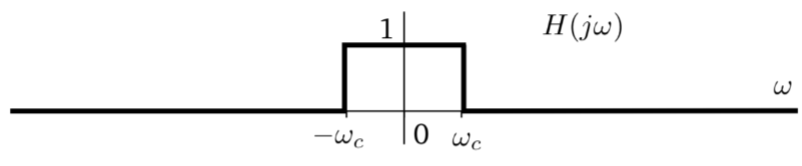
\includegraphics[width=\textwidth]{W7_5.png}
\end{center}
We call the region where frequencies are not suppressed (i.e., up to frequency $\omega_c$ for this ideal low pass filter) the "passband."  This filter can be represented as
\[H(j\omega) = \rect(\omega / (2\omega_c))\]
\begin{align*}
    \rect\left(\frac{t}{T}\right) &\llra T \cdot \sinc\left(\frac{\omega T}{2\pi}\right)
    \intertext{By duality:}
    \frac{1}{2\pi} T \cdot \sinc\left(\frac{t \cdot T}{2\pi}\right) &\llra \rect\left(\frac{\omega}{T}\right)
\end{align*}
Let $T = 2\omega_c$\dots
\begin{align*}  
    h(t) &= \frac{1}{2\pi} \cdot 2\omega_c \cdot \sinc\left(\frac{t \cdot 2 \omega_c}{2\pi}\right)\\
    \Aboxed{h(t) &= \frac{\omega_c}{\pi} \sinc\left(\frac{\omega_c}{\pi} \cdot t\right)}
\end{align*}
What are limitations of actually filtering this signal?
\begin{itemize}
    \item The impulse response is non-causal, i.e., it is nonzero for $t < 0$.  Hence, ideal low pass filtering the signal at time $t$ requires convolution with future signal, which might not be known to us.
    \item The filter impulse response has an infinite duration, and thus to convolve would take an infinite amount of time.  Realistically, $\sinc(\cdot)$ is close to zero as $|t|$ grows, so it could be truncated
    \item But even if we truncate it, we see that $\sinc(t)$ decays with an envelope of $1/t$ (since $\sinc(t) = \sin(\pi t) / \pi t$), and so the decay is relatively slow.  It would be better if the impulse response decayed faster, like $1/t^2$, etc.  This means the impulse response convolution requires less computation time.
\end{itemize}
\subsubsection*{A (less ideal) low pass filter}
Consider the following low pass filter, which is not ideal because it lets in some frequencies between $\omega_c$ and $2\omega_c$, albeit attenuated.  This region (from $[\omega_c, 2\omega_c]$) is sometimes called the \textit{transition band}.
\begin{center}
    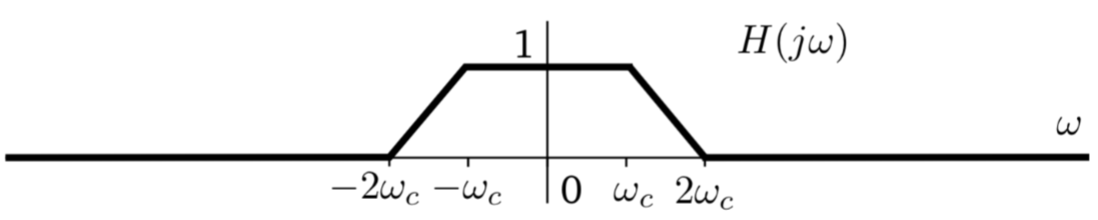
\includegraphics[width=\textwidth]{W7_6.png}
\end{center}
How do we write $H(j\omega)$ in a way that is amenable to a simple inverse Fourier transform using things we already know?
\begin{itemize}
    \item We write it as a convolution of two rectangles!
\end{itemize}
\[\rect\left(\frac{\omega}{3\omega_c}\right) * \rect\left(\frac{\omega}{\omega_c}\right)\]
Then, 
\begin{align*}
    H(j\omega) &= \rect\left(\frac{\omega}{3\omega_c}\right) * \rect\left(\frac{\omega}{\omega_c}\right)\\
    h_1(t) = \fourier^{-1}\left[\rect\left(\frac{\omega}{3\omega_c}\right)\right] &= \frac{3\omega_c}{2\pi} \sinc\left(\frac{3\omega_c}{2\pi}t\right)\\
    h_2(t) = \fourier^{-1}\left[\rect\left(\frac{\omega}{\omega_c}\right)\right] &= \frac{\omega_c}{2\pi} \sinc\left(\frac{\omega_c}{2\pi}t\right)\\
    \therefore \fourier[h_1(t) \cdot h_2(t)] &= \frac{1}{2\pi} H_1(j\omega) * H_2(j\omega)\\
    h(t) &= 2\pi \cdot h_1(t) \cdot h_2(t)\\
    &= \frac{3\omega_c^2}{2\pi} \cdot \sinc\left(\frac{3\omega_c t}{2\pi}\right) \cdot \sinc\left(\frac{\omega_c}{2\pi} t\right)
\end{align*} 
\subsubsection*{Ideal High Pass Filter}
The ideal high pass filter is:
\begin{center}
    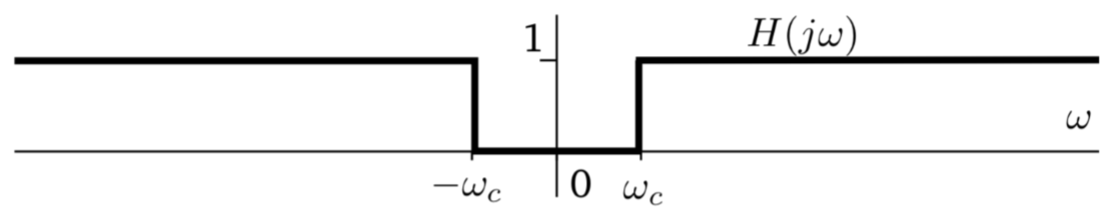
\includegraphics[width=\textwidth]{W7_7.png}
\end{center}
This can be written as 1 minus the ideal low pass filter, i.e.,
\[H(j\omega) = 1 - \rect(\omega / (2\omega_c))\]
Therefore, its impulse response is
\[h(t) = \delta(t) - \frac{\omega_c}{\pi} \sinc\left(\frac{\omega_c}{\pi}t\right)\]
This filter has the same limitations of the ideal low pass filter, with the additional inconvenience that we need to generate an approximate $\delta(t)$.
\begin{itemize}
    \item Can we get rid of the $\delta(t)$ in the high pass filter?
    \item How do we get around having a $\delta(t)$ in the impulse response?
\end{itemize}
\subsubsection*{Ideal Band Pass Filter}
The ideal band pass filter is:
\begin{center}
    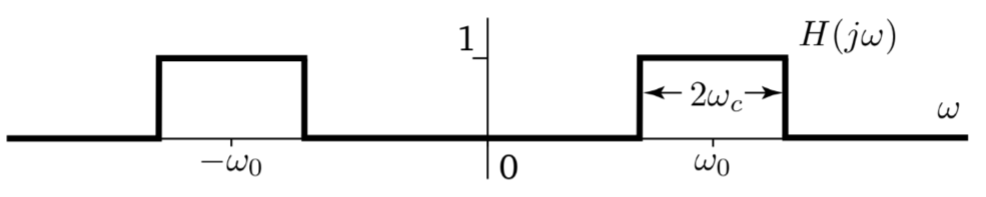
\includegraphics[width=\textwidth]{W7_8.png}
\end{center}
The frequency response of this filter is
\[H(j\omega) = \rect\left(\frac{\omega + \omega_0}{2\omega_c}\right) + \rect\left(\frac{\omega - \omega_0}{2\omega_c}\right)\]
\begin{align*}
    H(j\omega) &= \rect\left(\frac{\omega}{2\omega_c}\right) * \left[\delta(\omega - \omega_0) + \delta(\omega + \omega_0)\right]\\
    \fourier^{-1}\left[\rect\left(\frac{\omega}{2\omega_c}\right)\right] &= \frac{\omega_c}{\pi} \cdot \sinc\left(\frac{\omega_c}{\pi} t\right)\\
    \fourier^{-1}\left[\delta(\omega - \omega_0) + \delta(\omega + \omega_0)\right] &= \frac{1}{\pi} \cos(\omega_t)\\
    \fourier\left[f_1(t) \cdot f_2(t)\right] &= \frac{1}{2\pi} F_1(j\omega) + F_2(j\omega)\\
\end{align*}
\begin{align*}
    h(t) &= 2\pi \cdot \frac{\omega_c}{\pi} \cdot \sinc\left(\frac{\omega_c}{\pi}t\right) \cdot \frac{1}{\pi} \cos(\omega_0 t)\\
    &= 2 \cdot \cos(\omega_0 t) \cdot \left[\frac{\omega_c}{\pi} \sinc\left(\frac{\omega_c}{\pi}t\right)\right]
\end{align*}
The impulse response of the ideal band pass filter is:
\begin{center}
    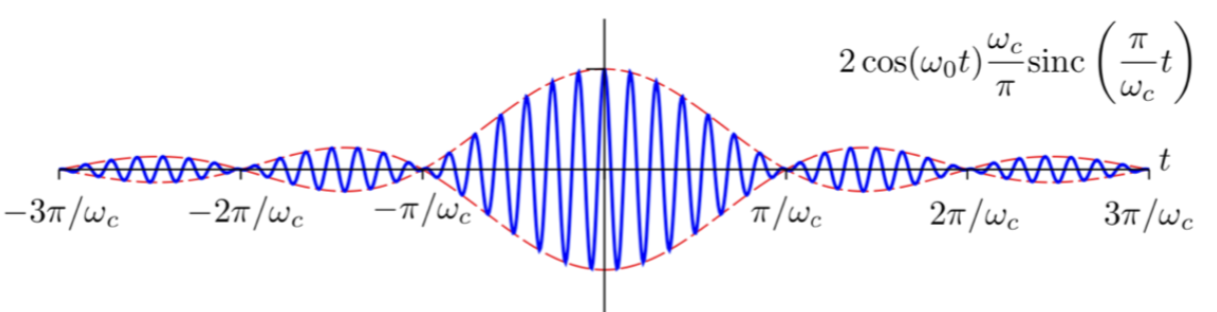
\includegraphics[width=\textwidth]{W7_9.png}
\end{center}
Hence, convolution with this impulse response extracts out frequencies in a range $\omega_0 \pm \omega_c$!  The same intuitions about using a transition band to make the filter more practical hold.
\subsection*{Example: AM Radio}
We previously talked about amplitude modulation (AM) which is used for e.g., AM radio.  We are now equipped to understand how it works.  Here is the problem setup:
\begin{itemize}
    \item Say we want to transmit a message signal, $m(t)$.
    \item To avoid interference and leverage the electromagnetic spectrum, we are given a frequency range over which we can transmit this signal.
    \item Anyone with knowledge of what frequency we are transmitting on can tune a receiver to receive the message signal, $m(t)$.
\end{itemize}
The fundamental idea of AM radio is to "multiply by a cosine".\\\\
When we do, the transmitted signal is $m(t) \cos(\omega_c t)$ with Fourier transform
\[\frac{1}{2} [M(j(\omega + \omega_c)) + M(j(\omega - \omega_c))]\]
Hence, multiplying by cosine creates copies of the signal at $\pm \omega_c$.\\\\
Let's show this mathematically.  If
\[\fourier[m(t) \cos(\omega_c t)] = \frac{1}{2} M(j(\omega + \omega_c)) + \frac{1}{2}M(j(\omega - \omega_c))\]
Then,
\begin{align*}
    \fourier[m(t) \cos^2(\omega_c t)] &= \frac{1}{2\pi} \left[\frac{1}{2} M(j(\omega + \omega_c)) + \frac{1}{2}M(j(\omega - \omega_c))\right] \cdots * [\pi \delta(\omega + \omega_c) + \pi\delta(\omega - \omega_c)]\\
    &= \frac{1}{4} \left[M(j(\omega + 2\omega_c)) + 2M(j\omega) + M(j(\omega - 2\omega_c))\right]\\
    &= \frac{1}{2} M(j\omega) + \frac{1}{4}M(j(\omega - 2\omega_c)) + \frac{1}{4}M(j(\omega + 2\omega_c))
\end{align*}
What if we demodulated by multiplying with a sine?  i.e.,
\[m(t)\cos(\omega_c t) \sin(\omega_c t)\]
It zeros the basebound replica.

\subsubsection*{What do we do after demodulation?}
We apply a low pass filter to get remove all replicas except the one we want (basebound).


\end{document}